\section{Applications}
\label{sec:applications}

Each application example is a notebook in the online material: We could have
one analysis as Python scripts instead of notebook in the online material. At
the start of this section, point to gammapy-paper repo on Github and say that
there’s a Binder where people can try the examples online.

TODO: mention other application examples (joint Crab paper, HESS validation
paper, HGPS, ...) here or in a subsection "other applications" at the end of
this section?

\subsection{Source detection}
\label{ssec:source-detection}

See Figure~\ref{fig:fermi_ts_map}.

Ref:~\citep{Stewart2009}

\begin{figure*}[t]
	\centering
	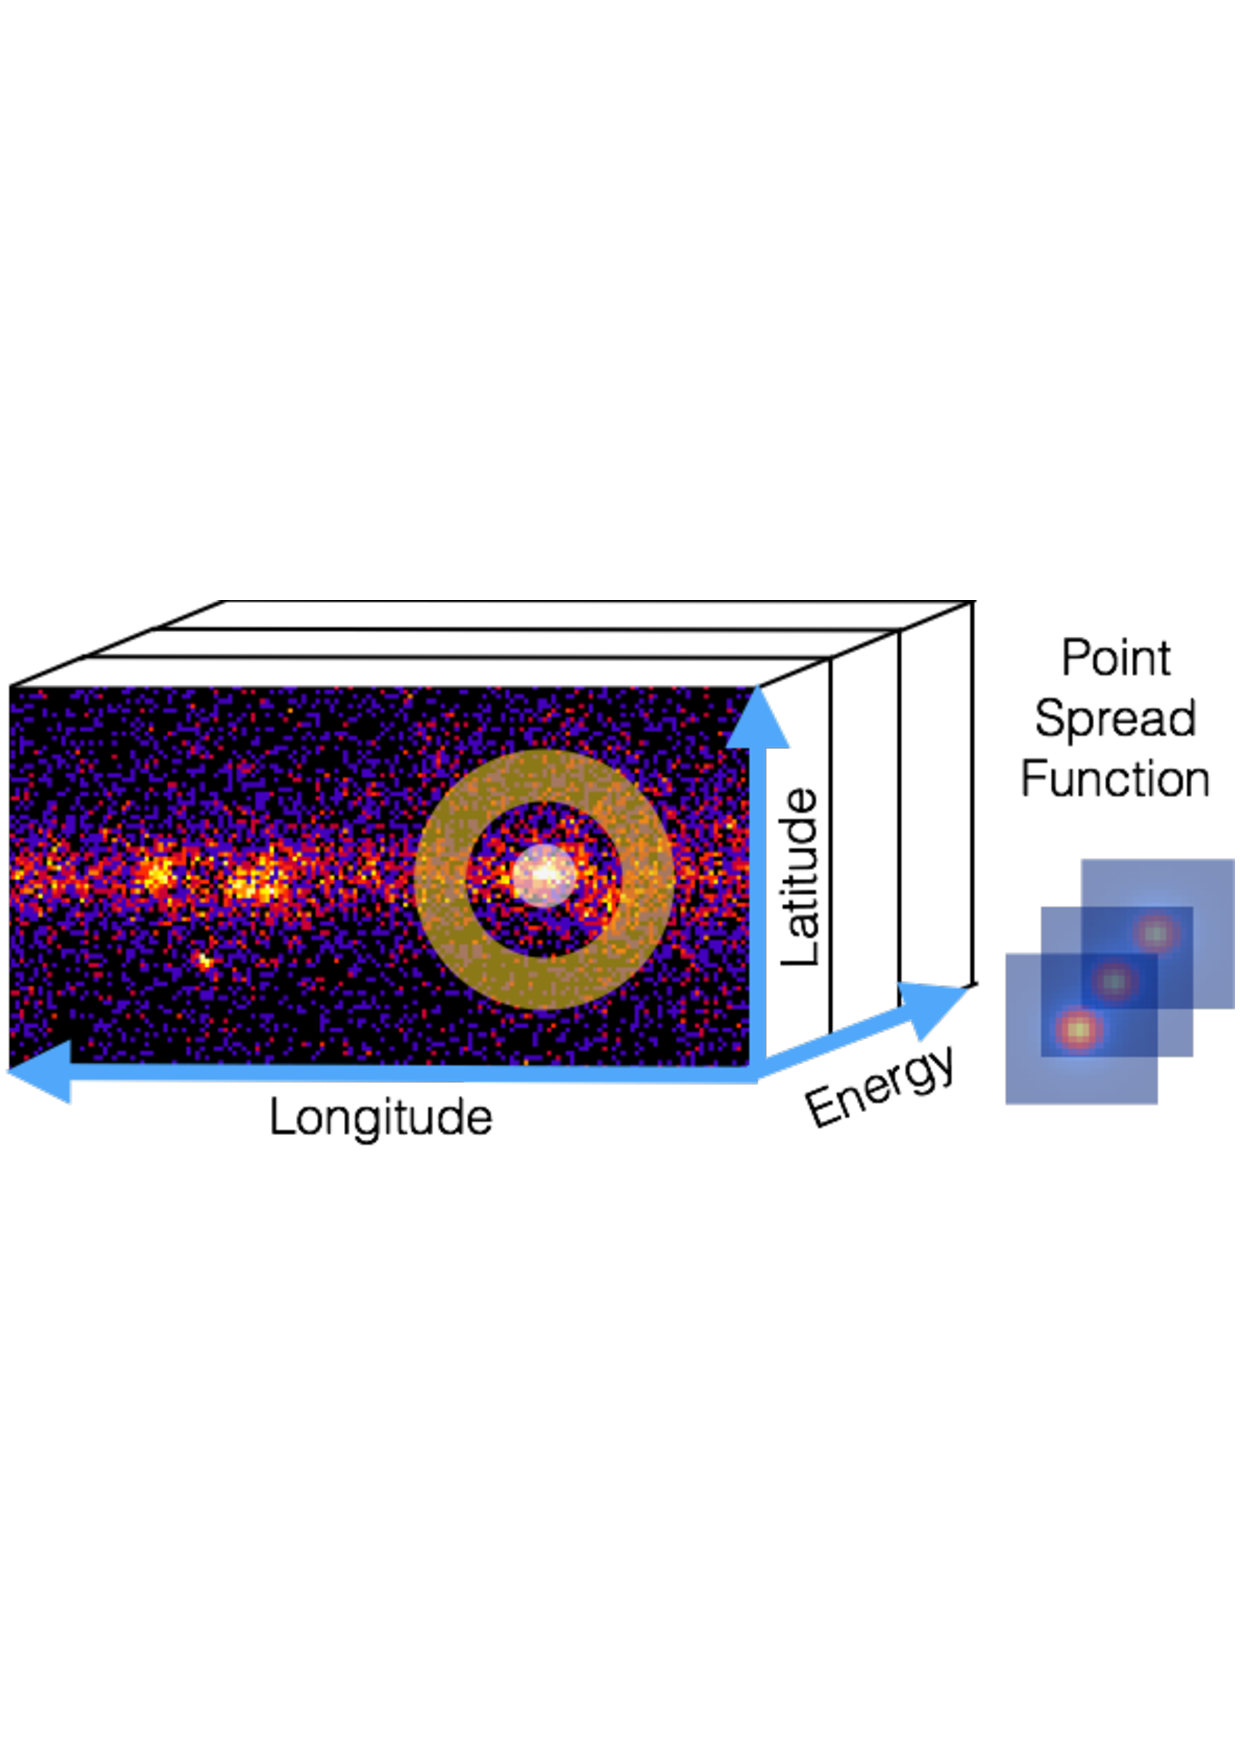
\includegraphics[width=0.8\textwidth]{static/gammapy-cube-analysis}
	\caption{
		Gammapy data model illustration. Binned analysis of lon-lat-energy cube data is
		supported via joint likelihood analysis of one image per energy bin.
		On-off-region based spectral analysis is supported as well. }
	\label{fig:data-model}
\end{figure*}

\subsection{Multi instrument analysis}
\label{ssec:multi-instrument-analysis}
